\documentclass[border=10pt]{standalone}
\usepackage{tikz}
\usepackage{amssymb}
\usepackage{fontspec}
\usetikzlibrary{decorations.markings,arrows.meta,positioning,calc}

% ---- Fonts (comment out if not available; falls back to Computer Modern) ----
% \setmainfont{EB Garamond}

\begin{document}
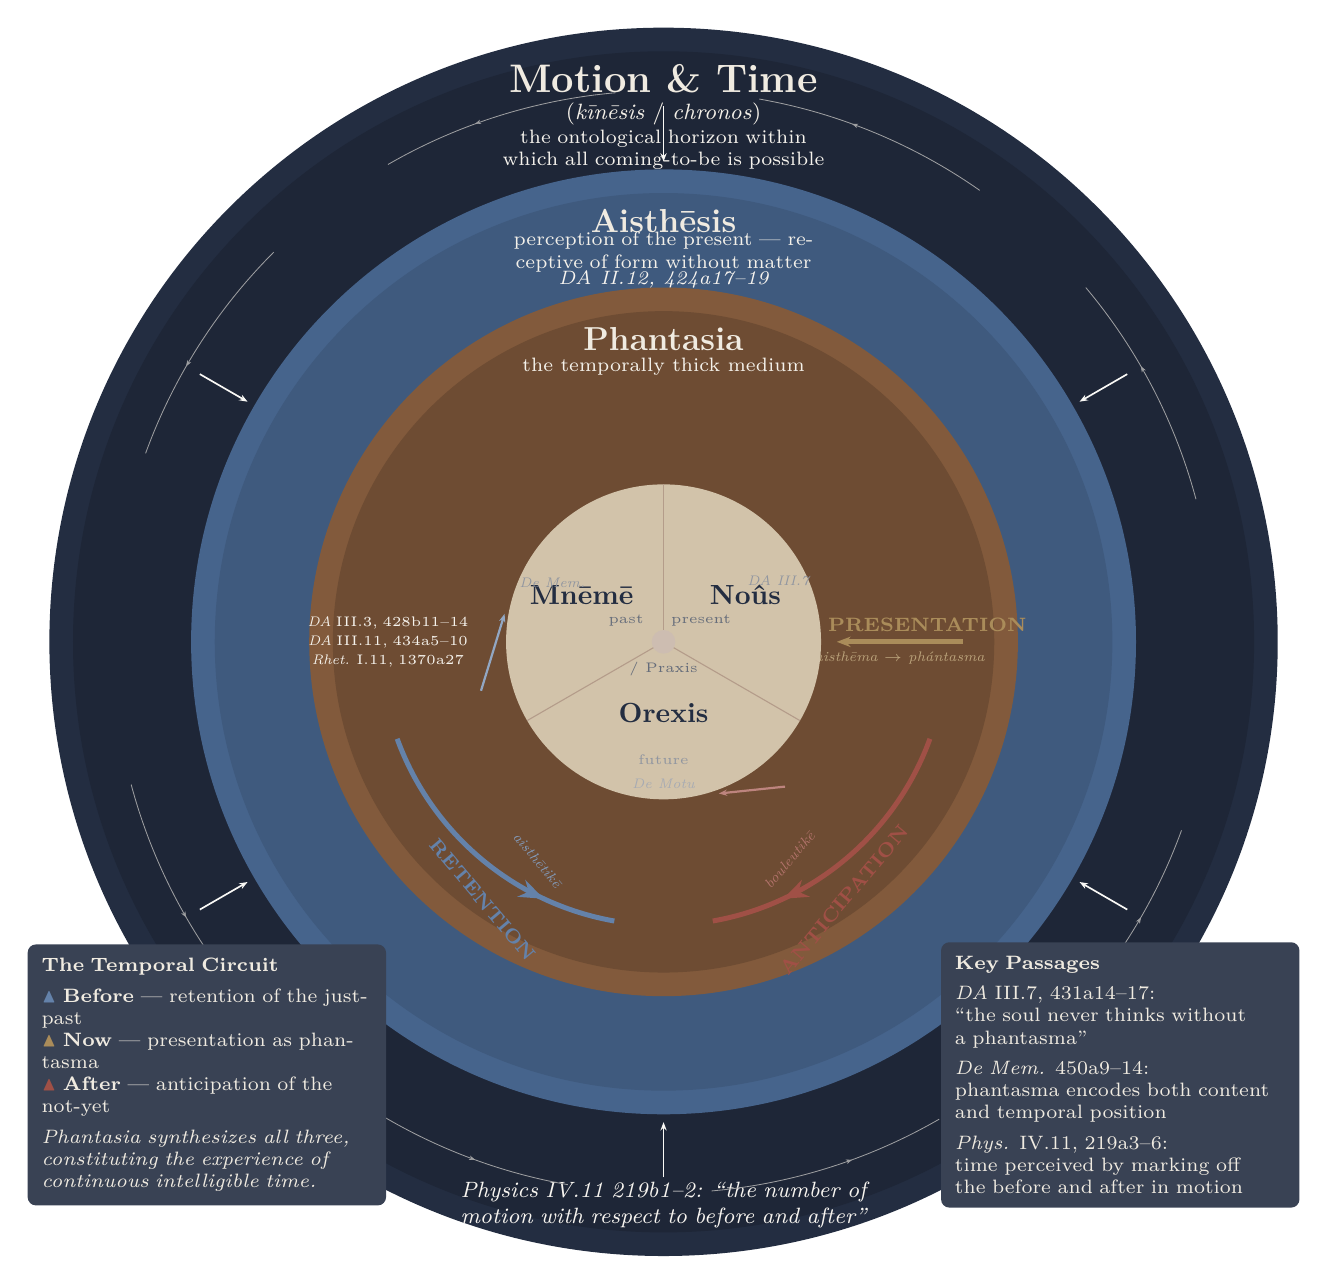
\begin{tikzpicture}[
    every node/.style={font=\small},
    >=Stealth,
]

% ============================================================================
% COLOR DEFINITIONS
% ============================================================================
\definecolor{horizoncolor}{RGB}{35,45,65}       % deep navy
\definecolor{aisthesiscolor}{RGB}{70,100,140}    % steel blue
\definecolor{phantasiacolor}{RGB}{130,90,60}     % warm bronze
\definecolor{corecolor}{RGB}{210,195,170}        % parchment
\definecolor{arrowretain}{RGB}{100,130,170}      % cool blue (past)
\definecolor{arrowpresent}{RGB}{170,140,90}      % gold (present)
\definecolor{arrowanticip}{RGB}{160,80,70}       % warm red (future)
\definecolor{labelcolor}{RGB}{240,235,225}       % off-white

% ============================================================================
% RING 0: MOTION & TIME — Ontological Horizon
% ============================================================================
\fill[horizoncolor] (0,0) circle (7.8cm);
\fill[horizoncolor!85!black] (0,0) circle (7.5cm);

% Horizon label (top)
\node[font=\Large\bfseries\scshape, text=labelcolor]
    at (0,7.15) {Motion \& Time};
\node[font=\footnotesize, text=labelcolor!80]
    at (0,6.7) {(\textit{k\={\i}n\={e}sis} / \textit{chronos})};
\node[font=\scriptsize, text=labelcolor!60, text width=6cm, align=center]
    at (0,6.25) {the ontological horizon within which all coming-to-be is possible};

% Horizon label (bottom)
\node[font=\footnotesize\itshape, text=labelcolor!50, text width=8cm, align=center]
    at (0,-7.15) {\textit{Physics} IV.11 219b1--2: ``the number of motion with respect to before and after''};

% Subtle motion indicators around the perimeter
\foreach \a in {15,55,95,135,195,235,275,315} {
    \draw[horizoncolor!40!labelcolor, line width=0.3pt,
          decoration={markings, mark=at position 0.6 with {\arrow[scale=0.5]{>}}},
          postaction={decorate}]
        (\a:7.0cm) arc (\a:\a+25:7.0cm);
}

% ============================================================================
% RING 1: AISTHESIS — Perceptual Contact Layer
% ============================================================================
\fill[aisthesiscolor] (0,0) circle (6.0cm);
\fill[aisthesiscolor!90!black] (0,0) circle (5.7cm);

% Aisthesis label
\node[font=\large\bfseries, text=labelcolor]
    at (0,5.35) {Aisth\={e}sis};
\node[font=\scriptsize, text=labelcolor!70, text width=5cm, align=center]
    at (0,4.95) {perception of the present --- receptive of form without matter};
\node[font=\scriptsize\itshape, text=labelcolor!50]
    at (0,4.6) {\textit{DA} II.12, 424a17--19};

% Permeability indicators (world's motion entering)
\foreach \a in {30,90,150,210,270,330} {
    \draw[labelcolor!30, line width=0.6pt, -{Stealth[length=3pt]}]
        (\a:6.8cm) -- (\a:6.1cm);
}

% ============================================================================
% RING 2: PHANTASIA — The Sustaining/Projecting Layer
% ============================================================================
\fill[phantasiacolor] (0,0) circle (4.5cm);
\fill[phantasiacolor!85!black] (0,0) circle (4.2cm);

% Phantasia label (centered top of ring)
\node[font=\large\bfseries, text=labelcolor]
    at (0,3.85) {Phantasia};
\node[font=\scriptsize, text=labelcolor!70]
    at (0,3.5) {the temporally thick medium};

% ---- THREE TEMPORAL VECTORS (the core of the argument) ----

% RETENTION arrow (curves backward/left) — past
\draw[arrowretain, line width=1.8pt,
      decoration={markings, mark=at position 0.75 with {\arrow[scale=0.8]{Stealth}}},
      postaction={decorate}]
    (200:3.6cm) arc (200:260:3.6cm);
\node[font=\scriptsize\bfseries, text=arrowretain, rotate=-50]
    at (235:4.0cm) {RETENTION};
\node[font=\tiny\itshape, text=arrowretain!80, rotate=-50]
    at (240:3.2cm) {aisth\={e}tik\={e}};

% PRESENTATION arrow (points inward) — present
\draw[arrowpresent, line width=1.8pt, -{Stealth[length=5pt]}]
    (0:3.8cm) -- (0:2.2cm);
\node[font=\scriptsize\bfseries, text=arrowpresent, rotate=0, anchor=south]
    at (0:3.35cm) {PRESENTATION};
\node[font=\tiny\itshape, text=arrowpresent!80, anchor=north]
    at (0:3.0cm) {aisth\={e}ma $\rightarrow$ ph\'{a}ntasma};

% ANTICIPATION arrow (curves forward/right) — future
\draw[arrowanticip, line width=1.8pt,
      decoration={markings, mark=at position 0.75 with {\arrow[scale=0.8]{Stealth}}},
      postaction={decorate}]
    (340:3.6cm) arc (340:280:3.6cm);
\node[font=\scriptsize\bfseries, text=arrowanticip, rotate=50]
    at (305:4.0cm) {ANTICIPATION};
\node[font=\tiny\itshape, text=arrowanticip!80, rotate=50]
    at (300:3.2cm) {bouleutik\={e}};

% Temporal synthesis label
\node[font=\tiny, text=labelcolor!60, text width=3cm, align=center]
    at (180:3.5cm) {\textit{DA} III.3, 428b11--14\\[1pt]\textit{DA} III.11, 434a5--10\\[1pt]\textit{Rhet.} I.11, 1370a27};

% ============================================================================
% INNER CORE — Three Sectors (Mneme, Nous, Orexis/Praxis)
% ============================================================================
\fill[corecolor] (0,0) circle (2.0cm);

% Dividing lines (three sectors)
\draw[phantasiacolor!60, line width=0.4pt] (0,0) -- (90:2.0cm);
\draw[phantasiacolor!60, line width=0.4pt] (0,0) -- (210:2.0cm);
\draw[phantasiacolor!60, line width=0.4pt] (0,0) -- (330:2.0cm);

% MNEME (upper-left sector — past-oriented)
\node[font=\normalsize\bfseries, text=horizoncolor] at (150:1.2cm) {Mn\={e}m\={e}};
\node[font=\tiny, text=horizoncolor!70, text width=1.8cm, align=center]
    at (150:0.55cm) {past};
\node[font=\tiny\itshape, text=horizoncolor!50] at (152:1.6cm) {\textit{De Mem.}};

% Retention arrow feeding mneme
\draw[arrowretain!70, line width=0.8pt, -{Stealth[length=3pt]}]
    (195:2.4cm) -- (170:2.05cm);

% NOUS (upper-right sector — present-oriented)
\node[font=\normalsize\bfseries, text=horizoncolor] at (30:1.2cm) {No\^{u}s};
\node[font=\tiny, text=horizoncolor!70, text width=1.8cm, align=center]
    at (30:0.55cm) {present};
\node[font=\tiny\itshape, text=horizoncolor!50] at (28:1.65cm) {\textit{DA} III.7};

% OREXIS / PRAXIS (bottom sector — future-oriented)
\node[font=\normalsize\bfseries, text=horizoncolor] at (270:0.9cm) {Orexis};
\node[font=\tiny, text=horizoncolor!70] at (270:0.35cm) {/ Praxis};
\node[font=\tiny, text=horizoncolor!50] at (270:1.5cm) {future};
\node[font=\tiny\itshape, text=horizoncolor!40] at (270:1.8cm) {\textit{De Motu}};

% Anticipation arrow feeding orexis
\draw[arrowanticip!70, line width=0.8pt, -{Stealth[length=3pt]}]
    (310:2.4cm) -- (290:2.05cm);

% Central node
\fill[phantasiacolor!40] (0,0) circle (0.15cm);

% ============================================================================
% ANNOTATION: The Temporal Circuit (bottom-left)
% ============================================================================
\node[font=\scriptsize, text=labelcolor, text width=4.2cm, align=left,
      fill=horizoncolor!90, rounded corners=3pt, inner sep=5pt]
    at (-5.8,-5.5) {%
    \textbf{The Temporal Circuit}\\[3pt]
    \textcolor{arrowretain}{$\blacktriangle$} \textbf{Before} --- retention of the just-past\\
    \textcolor{arrowpresent}{$\blacktriangle$} \textbf{Now} --- presentation as phantasma\\
    \textcolor{arrowanticip}{$\blacktriangle$} \textbf{After} --- anticipation of the not-yet\\[3pt]
    \textit{Phantasia synthesizes all three,}\\
    \textit{constituting the experience of}\\
    \textit{continuous intelligible time.}
    };

% ============================================================================
% ANNOTATION: Key citations (bottom-right)
% ============================================================================
\node[font=\scriptsize, text=labelcolor, text width=4.2cm, align=left,
      fill=horizoncolor!90, rounded corners=3pt, inner sep=5pt]
    at (5.8,-5.5) {%
    \textbf{Key Passages}\\[3pt]
    \textit{DA} III.7, 431a14--17:\\
    ``the soul never thinks without\\
    a phantasma''\\[3pt]
    \textit{De Mem.} 450a9--14:\\
    phantasma encodes both content\\
    and temporal position\\[3pt]
    \textit{Phys.} IV.11, 219a3--6:\\
    time perceived by marking off\\
    the before and after in motion
    };

\end{tikzpicture}
\end{document}
